\section{Markov Model}\label{sec:models}

Navigating through a web site can be seen as a sequence of states where a pair of states is connected. One can simulate a tree representation of the web site where the root of the tree will be the domain (main) page and the leafs the deepest path a user can reach.
\\[2ex]
This was the inspiration to represent the training data, we convert training data into a graph representation, we considered each fragment of the url as a one single state, then we created the edges with all the following url that are reached from that parent state, additionally, each node and edge contain the number of times that was transversed.  Such a number is converted into a probability measurement, making our model a Markov chain model.
\\[2ex]
One important consideration here was creating a Markov chain model for each domain, the reason is that we considered a session only when the user is inside the same domain, whenever the user changes from one domain to others, for instance domain.com to example.com, we don’t keep the the link between those domains and we just consider that switch as a closing session from domain.com and a new open session of example.com. Besides, representing the links among different domain could affect our prediction and make affect the probabilities of the whole graph, for example a user can frequently visit web site A and B, whenever user surfaces over web site A, the prediction must we making isolated of the others domains and a similar behaviour should happen when the user surfaces over web site B. Also when we improve our model, the new incoming data of web site must be only update its corresponding probabilities, without affect the others.
\\[2ex]
You can wondering if the size of the model with different Markov chain could be grown into an exponentially way, however because we are already filtered sites that are not relevant during the preprocessing section, we can ensure that we only compute the useful data for the Markov chain for every domain visited by the user.

\subsection{Model test}\label{subsec:model_test}

The first attempt to make predictions we used was using the Hidden Markov Model of the library hmmlearn, however we realised that such approach was out of the scope, we found that Hidden Markov Model is on the top of the Markov chain model, making prediction where are taking into account not only the probabilities of the edges but also the probabilities of extra attribute of the states, for instances on variable to predict the most likely deepest path could be the mood of the user.
\\[2ex]
As an alternative solution, we considered the idea of~\cite{article:markovmodel}, we thought that simple deep-first method is not the most accurate for this purpose. The goal of our model is not predict the most likely deepest path but also make the prediction as fast as possible, method hill climbing search in markov hill climbing model was implemented to achieve so.
\\[2ex]
Method hill climbing search is based  on the hill climbing search method, hill climbing method is setup with a memory of one node and works as follow:

\begin{enumerate}
  \item Receives the graph model and the current state/path were we need to predict, such path it is not limited to be the very first page of the web site
  \item Stores the current path
  \item Takes the next states connected to the current state
  \item Computes the delta between of the probabilities of the states, if such delta is greater of the confident interval such state is discarded.
  \item If there are more than one next possible state, takes the one with the highest transition probability and updates the current path
  \item Repeats step 3,4 and 5 until there is no next states of the current path or we discard all the next states in step 4.
\end{enumerate}

Step 4 is an important aspect of our model because we want the most deepest useful path to be predicted, for example, we can have the following Markov chain model of a given domain:

\begin{figure}[!htp]
    \centering
    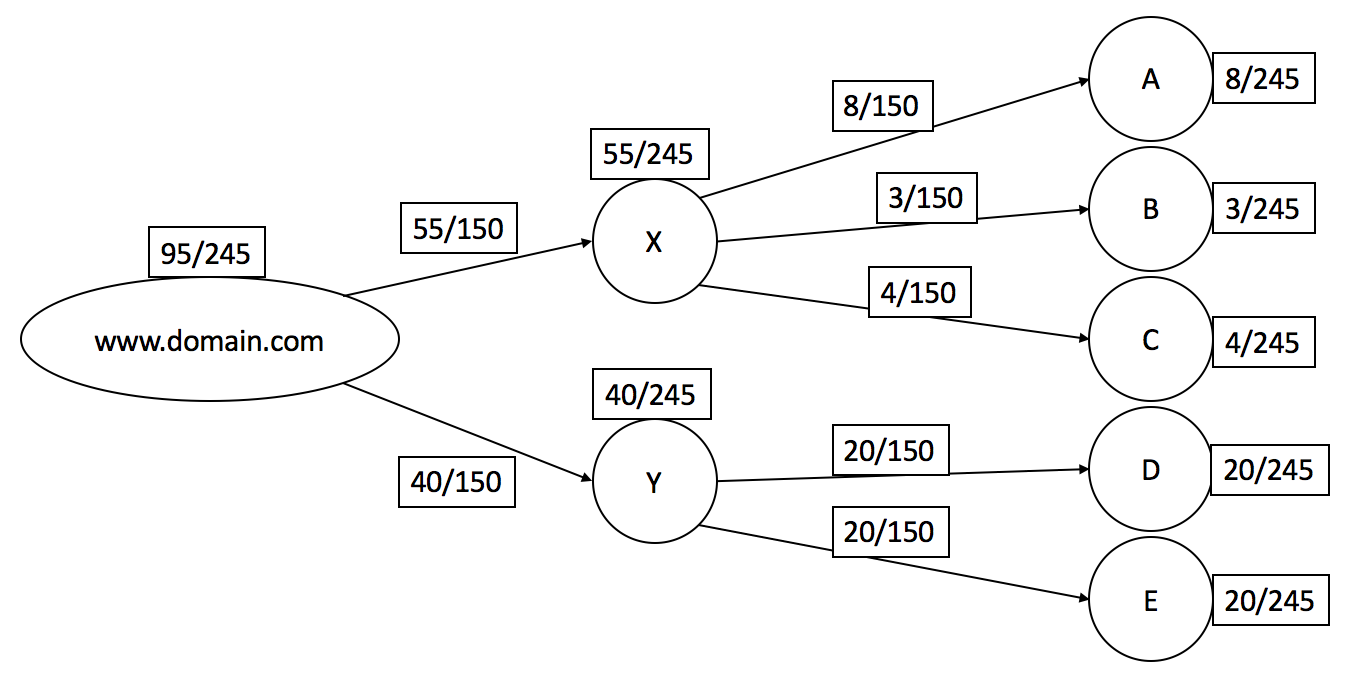
\includegraphics[width=\textwidth]{markov_chain}
    \caption{Markov chain model representation}\label{fig:markov_chain}
\end{figure}

www.domain.com represents the very first page of the web site, if the confident interval is setup as 1, the result of the search will be the path www.domain.com/X/A, however, according with the state probabilities, most of the time user stays in path www.domain.com/X, which probably it is more useful than www.domain.com/X/A. Now I we use our search method with a confident interval of 15\% the result of our search will be www.domain.com/X since the delta between state X and the next states connected with it are less that our confident interval.
\\[2ex]
When we ran our model with one of the possible scenarios, we kept track of those correct and incorrect predictions and then we computed the accuracy of our predictions, which is the total correct prediction divided by the total of predictions made. 
\\[2ex]
We also added a simulation of incremental learning in our model, each time we made a prediction we reinforced the graph with the real url that the user wants to visit according with our ground truth. We incremented the probabilities of such url (the correct path) in every iteration.

\subsection{Results}\label{subsec:results}
\\[2ex]
The result for the naive scenarios shows us that this method is not finest one. The more percentage of training data we give to our model, the more accuracy we get. This could interpreted as an overfitting of our data in our model. We can also need to consider that the data is split them randomly, in some user the accuracy of the data is high because of the set of training and testing data was split consistency, while in some user have the bad luck to have the training data and the test data with a very few relationship between them. This just confirmed our assumptions that this naive method is not the best for training and testing our model.
\\[2ex]
In the other hand, the result when we used the k fold cross validation was much consistent, if use the same confident interval with either incremental learning or non incremental learning and we test test our model, we almost obtain the same accuracy for each k fold configuration. After knowing that the k fold give us uniform result, we obtain the best accuracy where the confident interval is set in 20\%. Finally we obtained that the incremental learning increases slightly the accuracy of our model, in fact this is what we expected, since the amount of testing data is relatively small to actually learn from it. The more testing data we have, the more be can improve our model.